\section{Experiment}
\label{sec:shown_exp}
We wanted to test the hypothesis that a creativity support tool that offers adaptive conceptual guidance would help novices better utilize examples and improve creative outcomes than a tool that only provides non-adaptive examples.

\subsection{Method}

\subsubsection{Participants}
We recruited 24 novice participants (9 male, 15 female, median age = 22) through social media, mailing list advertisements, and the site UserTesting to evaluate our Wizard-of-Oz system. Similar to our interviews, we recruited novices that had familiarity with comics, but no formal education in art or professional experience in making comics. We also required participants to draw using a digital tablet with a stylus for ease of drawing. Half the participants were randomly assigned to the \textit{non-adaptive} condition while the other half was assigned to the \textit{adaptive} condition. The task asked participants to make a rough draft of a four-panel comic based on a randomly-assigned prompt from the interview study (\textsc{Penguin}, \textsc{Aliens}, or \textsc{Character} prompts). Four participants from each condition saw each of the three prompts. We encouraged black-and-white comics for simplicity, but using color was allowed. All one-hour sessions took place on the Zoom video conferencing platform, and participants received a USD \$25 gift card for their participation. 

\subsubsection{Procedure}
At the start of each study session, participants received a link to Sh{\"o}wn on Google Jamboard and were given a tutorial from the experimenter about Sh{\"o}wn’s features. \textit{Adaptive} condition participants created their comic in a version of Sh{\"o}wn with adaptive conceptual guidance where conceptual examples were presented selectively based on the heuristics described earlier. \textit{Non-adaptive} condition participants used an otherwise identical version of Sh{\"o}wn without adaptive conceptual guidance (the same conceptual examples were available via the example screens, but not selectively presented, similar to previous work with example galleries). All participants had access to the drawing helper because our main research question was about adaptive conceptual guidance versus non-adaptive examples. We chose to include the drawing helper for both conditions because Google Jamboard's Autodraw feature, which is the engine behind the drawing helper's icons, already exists within the tool itself.
Participants spent up to an hour drawing their comic while using a think-aloud protocol \cite{ericsson1984protocol}. At the end of the study session, participants answered post-interview questions about their process and thoughts on Sh{\"o}wn’s scaffolds. Following the study, we debriefed participants to inform them about the Wizard-of-Oz nature of the study.

\subsubsection{Measures}
We measured participants' behaviors and interactions with Sh{\"o}wn's features, such as the number of times participants used the drawing helper, viewed examples, and verbally expressed implementing concepts from the examples. We determined whether participants implemented examples either by their verbal expression of doing so or if they changed their panel after viewing examples. We also measured creative outcomes by gathering quality ratings of each comic from lay readers. We chose lay readers as raters (rather than experts) because lay readers are a large audience for comics, and because we wanted to capture overall story impact rather than technical quality, in line with the focus of both experts and novices in our interview study on narrative clarity.

Specifically, we measured comics in terms of clarity, creativity, and overall preference. In pairwise comparisons, raters from Mechanical Turk (61 unique Mechanical Turk workers) were sequentially presented with a pair of comics (two comics for the same prompt, one from each condition). For each pair, raters selected which comic they believed had more unique drawings and a more unique story (creativity), which comic had clearer drawings and a clearer story (clarity), and which comic they preferred overall. We separated drawing measures from story measures to account for potential individual differences in drawing ability. Pairing one comic from each condition for each prompt yielded 48 unique pairs (four \textit{non-adaptive} comics $\times$ four \textit{adaptive} comics $\times$ three prompts). Workers were paid USD \$1 to rate five pairs in sequence. Every pair received evaluations from at least five different raters, resulting in 306 total ratings.

\subsection{Results}

\begin{figure*}
  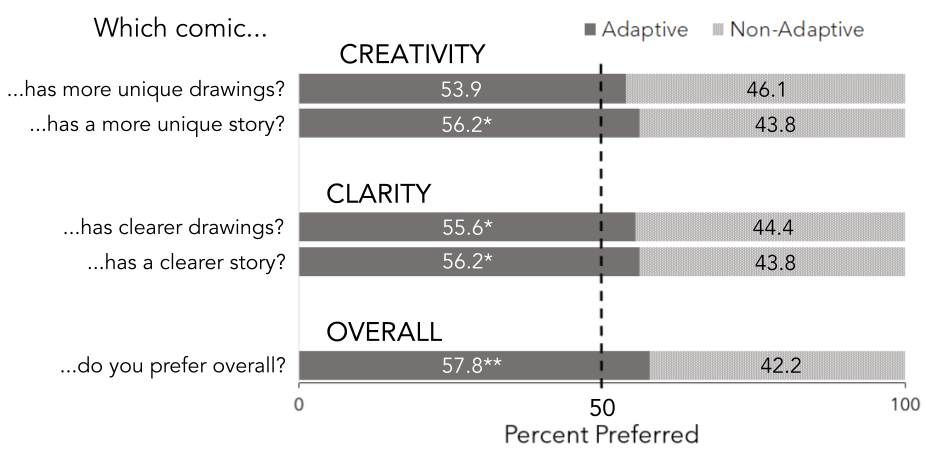
\includegraphics[width=\textwidth]{shown/figures/woz-results.png}
  \caption[\textit{Adaptive} condition ($n=12$) comics received significantly more preference ratings for more unique stories ($\chi^2=5.12, df=1, p<.05$), clearer drawings($\chi^2=3.91, df=1, p<.05$), clearer story ($\chi^2=5.12, df=1, p<.05$), and overall preference ($
\chi^2=7.87, df=1, p<.01$)]{\textit{Adaptive} condition ($n=12$) comics received significantly more preference ratings for more unique stories ($\chi^2=5.12, df=1, p<.05$), clearer drawings($\chi^2=3.91, df=1, p<.05$), clearer story ($\chi^2=5.12, df=1, p<.05$), and overall preference ($
\chi^2=7.87, df=1, p<.01$) than \textit{Non-adaptive} condition ($n=12$) comics. $*p<.05, **p<.01$}
  \label{fig:woz}
\end{figure*}

\subsubsection{Raters Preferred Adaptive Condition Comics Overall and for Most Other Measures}
Raters preferred \textit{adaptive} comics significantly more often than \textit{non-adaptive} comics overall (\textit{adaptive}=57.8\%, \textit{non-adaptive}=42.2\%, $
\chi^2=7.87, df=1, p<.01$) (Figure \ref{fig:woz}). In terms of clarity, raters preferred \textit{adaptive} comics more often when asked which had clearer drawings (\textit{adaptive}=55.6\%, \textit{non-adaptive}=44.4\%, $\chi^2=3.91, df=1, p<.05$) and which had clearer stories (\textit{adaptive}=56.2\%, \textit{non-adaptive}=43.8\%, $\chi^2=5.12, df=1, p<.05$). \textit{Adaptive} comics were also more often preferred when raters were asked which had more unique stories (\textit{adaptive}=56.2\%, \textit{non-adaptive}=43.8\%, $\chi^2=5.12, df=1, p<.05$). There was no significant difference in preference ratings for which comic had more unique drawings (\textit{adaptive}=53.9\%, \textit{non-adaptive}=46.1\%, $\chi^2=2.19, df=1, p=.14$). 
Figure \ref{fig:preferred} shows the most preferred comic for each measure as rated by the MTurk workers.

\subsubsection{Adaptive Conceptual Guidance Made Examples More Useful}
Sh{\"o}wn presented guidance at least three times to each \textit{adaptive} participant per session with a maximum of six times ($M=3.92$, $SD=0.90$). All \textit{adaptive} participants viewed at least one example screen at least one time while drawing, with an average of three times per session ($SD=1.13$). \textit{Adaptive} participants verbally expressed implementing concepts from examples an average of 2.17 times per session  ($SD=1.11$). In contrast, three \textit{non-adaptive} condition participants viewed examples, with an average of 0.67 examples viewed per session ($SD=1.23$)($t=4.84$, $df=21.8$, $p<.001$). 

\textit{Adaptive} participants mentioned that guidance served as inspiration, helping them think of new ways of showing their story they would not have otherwise realized. For example, P5 (\textit{adaptive}) noted, ``\textit{As I was going through I think I got into the same rhythm of what I wanted to show, and I think the [guidance] made me more cognizant of ways that I could switch things up. Like I don't think I would have thought of this last panel if I didn't get a nudge from those.}'' P16 (\textit{adaptive}), whose comic was the most preferred overall and for the most unique story, similarly stated, ``\textit{I think the [guidance] helped me consider different things. For example, for the 3rd panel, I wouldn't have considered doing a shot from the back of his head to show [the woman’s] point of view}'' (Figure \ref{fig:p16}). For the \textit{non-adaptive} participants who did view the examples, they also served as inspiration. P21 (\textit{non-adaptive}), whose comic was most preferred for having unique drawings, also cited the examples as helpful for their comic: ``\textit{[The examples] were kind of like a guide to give me a vocabulary for my intentions}.''

\begin{figure}[t]
  \hspace*{-1cm}%
  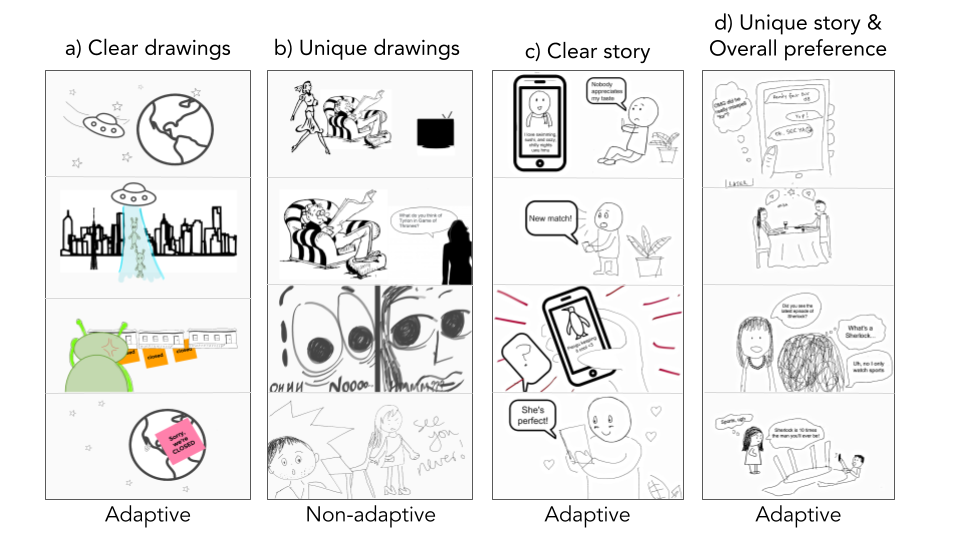
\includegraphics[width=\dimexpr\textwidth+2cm\relax]{shown/figures/preferred.png}
  \hspace*{-1cm}%
  \caption{The most preferred comics for each measure of clear drawings, unique drawings, clear story, unique story, and overall preference.}
  \label{fig:preferred}
\end{figure}

However, some \textit{non-adaptive} participants did not believe the examples were applicable. For example, P18 (\textit{non-adaptive}) stated, ``\textit{I already had an idea in mind so I didn’t really need the examples.}'' P15 (\textit{non-adaptive}) forgot the examples were available but wished he had used them after finishing his comic: ``\textit{I think I should have looked at [the examples] before I started drawing}.'' Similarly, although participants could proactively ask for guidance in the \textit{adaptive} condition, only two participants did so. One participant mentioned that he ``\textit{just wanted to see what suggestions were available}'' (P14, \textit{adaptive}). 

\subsubsection{Participants Wanted More Understandable Heuristics for Adaptive Conceptual Guidance}
The Wizard uses specific heuristics for displaying guidance. However, the heuristics Sh{\"o}wn used to decide when to show guidance, even if slightly off, could diminish the effectiveness of examples. Most felt the real-time guidance was useful: ``\textit{[The suggestions] were like a guidance for me. I don’t think I would go look at [the examples], so it was nice that they were shown throughout the drawing part}'' (P10, \textit{adaptive}). 
However, one participant wished guidance was presented at the beginning of drawing: ``\textit{I think these come a bit too late for me to use them because they're sparsed in between while I'm drawing. For example, the perspective one, I thought `oh, I should've used this earlier,' but the information just came a bit too late for me to use}'' (P6, \textit{adaptive}). 
This suggests that guidance heuristics should not be ``one-size-fits-all'' but rather allow users to adjust them based on perceived usefulness.

Some \textit{adaptive} participants also thought the timing and reasoning for presenting certain guidance was opaque. 
They wanted to know more about why particular advice was being given at a particular moment. P24 (\textit{adaptive}) stated, ``\textit{The suggestions were helpful, but it wasn't clear why that suggestion was being given. Like for the transition one, it could be that my transition isn't the best one I could use for my viewer or it could just be helping me get started so it wasn't clear why it was giving me those suggestions}.''
While adaptive conceptual guidance helped participants better understand examples, clarity around what the system is responding to would help users decide between many possible valid uses of those examples.

\begin{figure}[b!]
  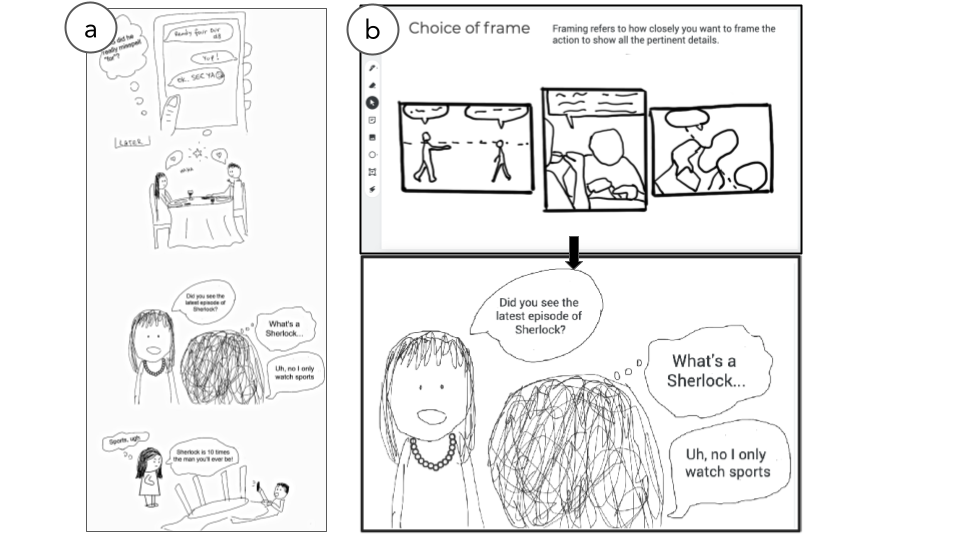
\includegraphics[width=\textwidth]{shown/figures/p16.png}
  \caption{a) This comic was created using Sh{\"o}wn's adaptive conceptual guidance. b) The participant cited that seeing a relevant example inspired the composition of the third panel of the comic.}
  \label{fig:p16}
\end{figure}

\subsubsection{The Drawing Helper Shifted Focus from Details to Story}
We tracked user interactions with the drawing helper to understand how people used this feature and how it possibly interacted with example use. Participants in both conditions used the drawing helper frequently, with an average of 4.67 times ($SD=2.87$) per session for \textit{adaptive} participants and 5.67 times ($SD=4.68$) for \textit{non-adaptive} participants ($t=-0.63$, $df=18.3$, $p=.54$). In some cases, the drawing helper made drawing objects---particularly repeated objects---less tedious. For example, P24 (\textit{adaptive}) used the drawing helper to draw a phone screen that would be consistent across all panels. P11 (\textit{non-adaptive}) felt the drawing helper did indeed help him focus less on details: ``\textit{I thought [the drawing helper] was really cool, especially for like tables or chairs or to hash out the overall setting so you can just focus on the other stuff.}'' P21 (\textit{non-adaptive}) thought the drawing helper was useful for showing her intended vision: ``\textit{I could just tell [the drawing helper] my vision, and it would bring up things that are relevant}.'' 
Our findings suggest that the concreteness provided by tools like the drawing helper may complement the efficacy of strategies like adaptive conceptual guidance. 

However, a few participants felt limited in their creativity with the drawing helper. One participant noted an over-reliance on the drawing helper rather than sketching, stating, ``\textit{I kinda became too dependent on [the drawing helper]. Normally, I would just draw it out quickly, but I want to see what the system can do...With the tool, I think if the system can do this for me, and it's perfect the first time, I try to see how I can fit my idea to what the system can do}'' (P15, \textit{non-adaptive}). 
Another participant felt that the simplicity of the drawing helper's sketches did not allow them to completely show their vision: ``\textit{It was pretty limited in what it could show. Like I couldn't do perspectives or angles with the basic icons I was given}'' (P12, \textit{adaptive}). 
These observations corroborate the fact that we found no significant difference in visual creativity across the two conditions ($\chi^2=2.20, df=1, p=.14$).
Three participants did not use the drawing helper or only used it once because, as one participant stated, ``\textit{It might have been more helpful if I was drawing something more complex, but it was just easier to draw it on my own}'' (P13, \textit{non-adaptive}). 